% Options for packages loaded elsewhere
\PassOptionsToPackage{unicode}{hyperref}
\PassOptionsToPackage{hyphens}{url}
%
\documentclass[
]{article}
\usepackage{amsmath,amssymb}
\usepackage{lmodern}
\usepackage{iftex}
\ifPDFTeX
  \usepackage[T1]{fontenc}
  \usepackage[utf8]{inputenc}
  \usepackage{textcomp} % provide euro and other symbols
\else % if luatex or xetex
  \usepackage{unicode-math}
  \defaultfontfeatures{Scale=MatchLowercase}
  \defaultfontfeatures[\rmfamily]{Ligatures=TeX,Scale=1}
\fi
% Use upquote if available, for straight quotes in verbatim environments
\IfFileExists{upquote.sty}{\usepackage{upquote}}{}
\IfFileExists{microtype.sty}{% use microtype if available
  \usepackage[]{microtype}
  \UseMicrotypeSet[protrusion]{basicmath} % disable protrusion for tt fonts
}{}
\makeatletter
\@ifundefined{KOMAClassName}{% if non-KOMA class
  \IfFileExists{parskip.sty}{%
    \usepackage{parskip}
  }{% else
    \setlength{\parindent}{0pt}
    \setlength{\parskip}{6pt plus 2pt minus 1pt}}
}{% if KOMA class
  \KOMAoptions{parskip=half}}
\makeatother
\usepackage{xcolor}
\usepackage[margin=1in]{geometry}
\usepackage{longtable,booktabs,array}
\usepackage{calc} % for calculating minipage widths
% Correct order of tables after \paragraph or \subparagraph
\usepackage{etoolbox}
\makeatletter
\patchcmd\longtable{\par}{\if@noskipsec\mbox{}\fi\par}{}{}
\makeatother
% Allow footnotes in longtable head/foot
\IfFileExists{footnotehyper.sty}{\usepackage{footnotehyper}}{\usepackage{footnote}}
\makesavenoteenv{longtable}
\usepackage{graphicx}
\makeatletter
\def\maxwidth{\ifdim\Gin@nat@width>\linewidth\linewidth\else\Gin@nat@width\fi}
\def\maxheight{\ifdim\Gin@nat@height>\textheight\textheight\else\Gin@nat@height\fi}
\makeatother
% Scale images if necessary, so that they will not overflow the page
% margins by default, and it is still possible to overwrite the defaults
% using explicit options in \includegraphics[width, height, ...]{}
\setkeys{Gin}{width=\maxwidth,height=\maxheight,keepaspectratio}
% Set default figure placement to htbp
\makeatletter
\def\fps@figure{htbp}
\makeatother
\setlength{\emergencystretch}{3em} % prevent overfull lines
\providecommand{\tightlist}{%
  \setlength{\itemsep}{0pt}\setlength{\parskip}{0pt}}
\setcounter{secnumdepth}{-\maxdimen} % remove section numbering
\ifLuaTeX
  \usepackage{selnolig}  % disable illegal ligatures
\fi
\IfFileExists{bookmark.sty}{\usepackage{bookmark}}{\usepackage{hyperref}}
\IfFileExists{xurl.sty}{\usepackage{xurl}}{} % add URL line breaks if available
\urlstyle{same} % disable monospaced font for URLs
\hypersetup{
  pdftitle={Ailanthus altissima},
  pdfauthor={María Luisa Campón Amado},
  hidelinks,
  pdfcreator={LaTeX via pandoc}}

\title{Ailanthus altissima}
\author{María Luisa Campón Amado}
\date{2023-05-17}

\begin{document}
\maketitle

{
\setcounter{tocdepth}{4}
\tableofcontents
}
\begin{figure}
\centering
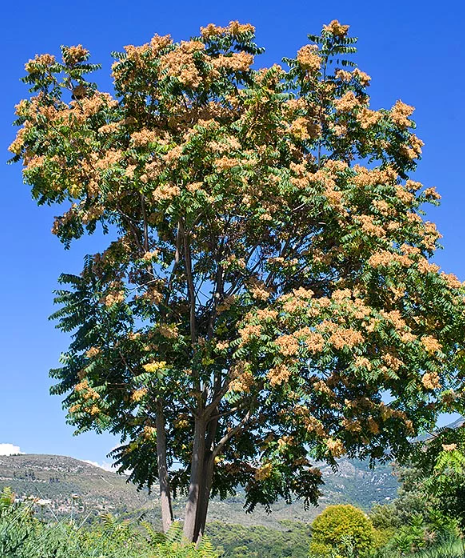
\includegraphics{C:/Users/Usuario/Desktop/practicaR/ailanthus.PNG}
\caption{\emph{Ailanthus altissima}}
\end{figure}

\hypertarget{descripciuxf3n}{%
\section{\texorpdfstring{\textbf{DESCRIPCIÓN}}{DESCRIPCIÓN}}\label{descripciuxf3n}}

Árbol que alcanza los 30 m de altura, de corteza lisa y grisácea, cuyo
tronco puede recordar a la pata de un elefante. Las hojas son muy
grandes, de hasta casi un metro de longitud, caducas, alternas y
compuestas por un número impar de hojuelas (imparipinnadas), que le dan
un aspecto plumoso. El margen de las hojuelas es irregular, a menudo con
lóbulos en la base, y tienen la característica de que huelen mal al ser
machacadas, por lo que a veces se denomina a este árbol malhuele. Las
flores masculinas y femeninas por lo general salen en distintos pies de
planta, con lo cual hay árboles macho y árboles hembra. Los frutos son
secos y tienen una semilla del tamaño de una lenteja rodeada de un ala
membranosa alargada que le sirve para la dispersión por el viento
(sámaras). Cuando maduran se retuercen un poco al secarse.

\hypertarget{ecologuxeda}{%
\section{\texorpdfstring{\textbf{ECOLOGÍA}}{ECOLOGÍA}}\label{ecologuxeda}}

Aparece aislado o en rodales e incluso llega a formar bosquetes. Se
asilvestra en cunetas, eriales, linderos, vías férreas, cultivos
abandonados, escombreras, vaguadas y fondos de valle. Es una planta muy
adaptable; resiste bien la contaminación y la sequía y medra sobre
cualquier tipo de suelo, pero sufre mucho con las heladas fuertes.
Germina con mucha facilidad de semilla y se extiende también por brotes
radicales, al punto de que se la puede ver incluso saliendo por grietas
de muros y rejas de alcantarillas. Necesita mucha luz y crece desde el
nivel del mar hasta los 1500 m.

\hypertarget{distribuciuxf3n}{%
\section{\texorpdfstring{\textbf{DISTRIBUCIÓN}}{DISTRIBUCIÓN}}\label{distribuciuxf3n}}

Árbol originario del sudeste de Asia que se ha naturalizado en muchas
regiones del mundo. En nuestro territorio aparece en todas las
provincias, a veces como ornamental y a menudo asilvestrado, llegando a
convertirse en especie invasora en muchos lugares. Está incluido en el
Atlas de las plantas alóctonas invasoras en España.

\begin{figure}
\centering
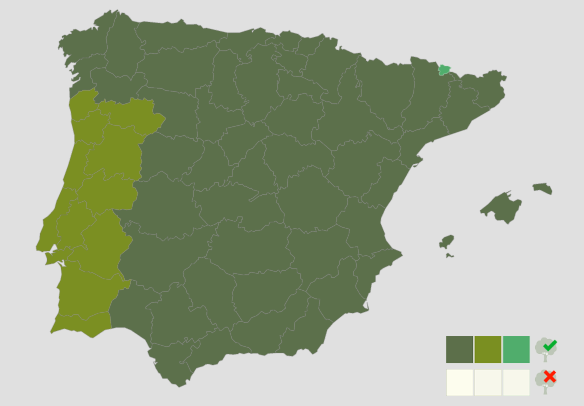
\includegraphics{C:/Users/Usuario/Desktop/practicaR/distribucionailanto.PNG}
\caption{Distribucion del ailanto en España}
\end{figure}

\hypertarget{estudios-del-ailanto-en-madrid}{%
\subsection{\texorpdfstring{\textbf{ESTUDIOS DEL AILANTO EN
MADRID}}{ESTUDIOS DEL AILANTO EN MADRID}}\label{estudios-del-ailanto-en-madrid}}

\hypertarget{material-y-muxe9todos}{%
\subsubsection{\texorpdfstring{\emph{Material y
métodos}}{Material y métodos}}\label{material-y-muxe9todos}}

Analizaron la evolución de Ailanthus altissima en la Comunidad de Madrid
desde su introducción hasta la actualidad. Para ello utilizaron varias
fuentes de información:

\begin{enumerate}
\def\labelenumi{\alph{enumi})}
\item
  \textbf{Bibliografía}
\item
  \textbf{Bases de datos}
\item
  \textbf{Herbarios}
\item
  \textbf{Prospecciones de 1992}
\end{enumerate}

Además se realizaron una búsqueda de bibliografía sobre la especie, para
analizar sus características, fisiología y ecología, que permita
analizar los mecanismos y vías de expansión de la especie en el
territorio estudiado.

\hypertarget{resultados}{%
\subsubsection{\texorpdfstring{\emph{Resultados}}{Resultados}}\label{resultados}}

\begin{enumerate}
\def\labelenumi{\alph{enumi})}
\tightlist
\item
  \textbf{Hasta 1979}: Se cultivaba en jardines como especie ornamental.
  Se obtuvo que había registros de la especie en 2 cuadrículas UTM de
  10x10 de las 115 que abarcaban la Comunidad de Madrid.
\end{enumerate}

\begin{figure}
\centering
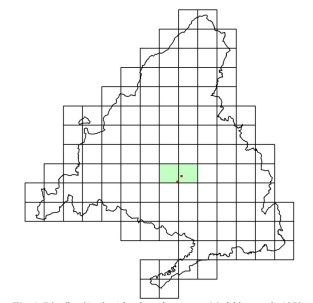
\includegraphics{C:/Users/Usuario/Desktop/practicaR/Figura1.PNG}
\caption{Distribución de \emph{Ailanthus altissima} en Madrid antes de
1979}
\end{figure}

\begin{enumerate}
\def\labelenumi{\alph{enumi})}
\setcounter{enumi}{1}
\tightlist
\item
  \textbf{1980-1999}: A partir de 1980 comienzan a encontrarse más citas
  de ailanto en Madrid. Hasta 1999 había registros de la especie en 15
  cuadrículas UTM de 10x10. Las prospecciones realizadas en 1992
  muestran sin embargo que la distribución de la especie entonces era ya
  entonces mucho más amplia, abarcando 45 cuadrículas UTM de 10×10, con
  citas en 67 cuadrículas de 1×1.
\end{enumerate}

\begin{figure}
\centering
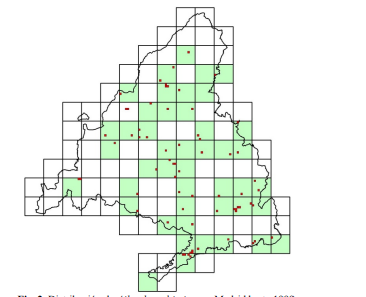
\includegraphics{C:/Users/Usuario/Desktop/practicaR/Figura2.PNG}
\caption{Distribución de \emph{Ailanthus altissima} en Madrid hasta
1999}
\end{figure}

\begin{enumerate}
\def\labelenumi{\alph{enumi})}
\setcounter{enumi}{2}
\tightlist
\item
  \textbf{2000-2019}: Nuestros resultados para 2019 muestran la
  presencia de la especie en 88 cuadrículas UTM de 10, un 76,5 \% del
  total estudiado, aunque un porcentaje mucho mayor en superficie, ya
  que las cuadrículas sin citas son casi todas perimetrales, algunas con
  una superficie madrileña muy reducida; dentro de ellas, hay registros
  en 948 cuadrículas de 1×1. En consecuencia, la presencia de la especie
  ha sufrido un gran incremento en las últimas décadas, estando presente
  en la mayoría de municipios de la región.
\end{enumerate}

\begin{figure}
\centering
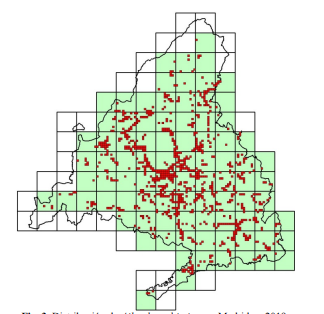
\includegraphics{C:/Users/Usuario/Desktop/practicaR/Figura3.PNG}
\caption{Distribución de \emph{Ailanthus altissima} en Madrid en 2019}
\end{figure}

\hypertarget{conclusiones}{%
\subsubsection{\texorpdfstring{\emph{Conclusiones}}{Conclusiones}}\label{conclusiones}}

El ailanto invade gran parte del territorio de la Comunidad de Madrid,
estando en una fase expansiva en las últimas décadas. Aunque su
principal vía de expansión son las carreteras, cada vez coloniza más
cauces fluviales, y hay casos puntuales de invasión de otras comunidades
naturales. Todo apunta a que está invasión va a continuar en el tiempo,
existiendo un importante riesgo de infestación en riberas e incluso en
bosques de frondosas de la Sierra a medio o largo plazo. La ausencia de
una cartografía detallada de distribución de esta especie, y más aún la
publicación de mapas que han infravalorado su presencia, han podido
llevar a minimizar un problema que en la actualidad es importante, y
exige tomar medidas. La administración autonómica ha desarrollado
actuaciones puntuales de erradicación en espacios naturales protegidos
en los últimos años, pero serían precisas acciones más amplias y
ambiciosas para mantener áreas libres de ailanto dentro de la región.
Las única especies que compite de forma eficaz con el ailanto son
precisamente otras invasoras, Ulmus pumila, Robinia pseudoacacia y
Gleditsia triacanthos. Su presencia en Madrid, sobre todo de la primera
especie, es muy elevada, precisando una mayor atención, ya que también
se están infravalorando sus riesgos. La cartografía de especies
invasoras es una herramienta esencial para su control, y debería
generalizarse, y actualizarse de forma periódica.

\begin{longtable}[]{@{}lll@{}}
\toprule()
Column 1 & Column 2 & Column 3 \\
\midrule()
\endhead
10 & 45 & 75 \\
\bottomrule()
\end{longtable}

data(mtcars) head(mtcars) table(mtcars\(cy1) barplot(table(mtcars\)cy))

\end{document}
